\documentclass[../th_cyber_warfare_distilled.tex]{subfiles}
 
\begin{document}
\chapter{ลักษณะพื้นที่การรบและแนวทางการใช้กำลัง}
 หลักนิยมการใช้กำลังเป็นแนวคิดที่ใช้กำหนดทิศทางการใช้กำลังรบเพื่อสนับสนุนวัตถุประสงค์ของชาติ การพัฒนาหลักนิยมจึงต้องคำนึงถึงปัจจัยสำคัญหลายประการดังแสดงในภาพที่ \ref{figure:war_doctrine} จะเห็นว่าปัจจัยสำคัญในการกำหนดหลักนิยมพื้นฐานของกำลังรบใดๆจะต้องสอดคล้องกับมุ่งประสงค์ของชาติ ผลประโยชน์ของชาติ ตลอดจนประวัติศาสตร์ทางทหาร บทเรียนจากการรบ หลักนิยมชาติอื่นๆ ฯลฯ 

\begin{figure}
	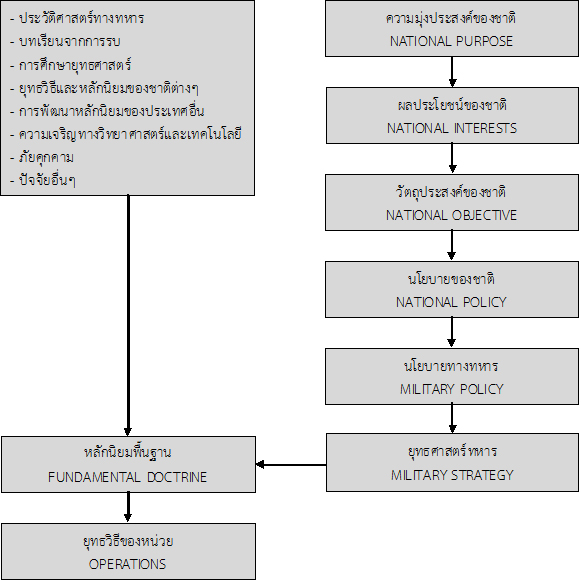
\includegraphics[scale=.65]{figure_war_doctrine.jpg}
	\centering
	\caption{ปัจจัยกำหนดหลักนิยม}
	\label{figure:war_doctrine}
\end{figure}


แม้ว่าจุดมุ่งหมายของการรบทางบก ทางทะเล และทางอากาศมีความคล้ายคลึงกันโดยมีความต้องการหลักๆเพื่อ ยึดพื้นที่ (Command) การควบคุมพื้นที่ (Control) หรือการปฏิเสธการใช้ประโยชน์ของพื้นที่ๆนั้นๆจากฝ่ายตรงข้าม (Denial) โดยการก้าวเข้าสู่สภาวะสงครามในการรบทางบก ทางทะเล และทางอากาศมีความตรงไปตรงมาโดยมักเริ่มขึ้นเมื่อกำลังของแต่ละฝ่ายเคลื่อนเข้าหากัน เพื่อยึดครอง ควบคุม หรือปฏิเสธการใช้ประโยชน์เหนือพื้นที่นั้นๆจากฝ่ายตรงข้ามด้วยกองกำลังของตน บนหรือในยุทธบริเวณนั้นๆ แต่สงครามไซเบอร์คุณลักษณะแตกต่างจากพื้นที่การรบอื่นๆอย่างมีนัยสำคัญ

\section{สงครามทางบก}
\paragraph{สงครามทางบก}
การดำเนินกลยุทธบนพื้นที่ทางบกมีมาควบคู่กับการวิวัฒนาการของมนุษย์ โดยอาวุธ ยุทธวิธีและการดำเนินกลยุทธของการทำการรบทางบกได้รับการพัฒนามาอย่างต่อเนื่อง นับตั้งแต่การขว้างปาหิน พัฒนาเป็นหอก ธนู เครื่องยิง ระเบิด ปืน ปืนใหญ่ ปืนกล รถถัง และกล่าวได้ว่าการพัฒนาของอาวุธชนิดต่างๆส่งผลโดยตรงต่อหลักนิยม ยุทธวิธีและการจัดกำลังซึ่งจะต้องถูกพัฒนาให้เหมาะสมกับอาวุธในแต่ละแบบ โดยมีแนวคิดพื้นฐานในการแบ่งมอบการบังคับบัญชาให้หน่วยรองและควบคุมการปฏิบัติ (Chain of Command and Span of Control) สำหรับการรบในยุคปัจจุบันจะพบว่าการใช้กำลังเพื่อทำการรบทางบกจะมีลักษณะเป็นการจัดกำลังผสมเหล่าที่ผนึกกำลังรบที่มีอำนาจการยิง และสามารถดำเนินกลยุทธด้วยการจู่โจม รวดเร็ว รุนแรง สามารถเอาชนะกำลังรถถังและยานเกราะ และมีส่วนยิงสนับสนุนจากอาวุธยิงสนับสนุน เช่นการจัดกองพันรบผสมเหล่าดังภาพที่ \ref{figure:combined_army_battalion} แสดงการจัดกองพันผสมซึ่งประกอบด้วยกองร้อยรถถัง กองร้อยรถสายพาน กองร้อยรถสายพานลาดตระเวณ และทหารราบ เพื่อปฏิบัติการรบด้ยวิธีรุก รับ และร่นถอยได้อย่างอ่อนตัวและมีประสิทธิภาพ และเมื่อพิจารณาประวัติศาสตร์สงครามที่ผ่านๆมาจะเห็นว่าการยุทธในปัจจุบันต่างก็มีการใช้กองกำลังผสมเหล่าในการทำการรบ
\begin{figure}
	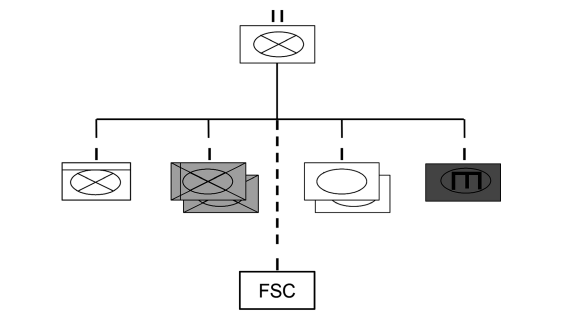
\includegraphics[scale=0.5]{figure_land_doctrine.png}
	\centering
	\caption{การจัดหน่วยระดับกองพันผสม}
	\label{figure:combined_army_battalion}
\end{figure}

\section{สงครามทางเรือ}
\paragraph{สงครามทางเรือ}
เมื่อพิจารณาพื้นที่ปฏิบัติการของการยุทธทางเรือจะพบว่าพื้นที่การยุทธมีอาณาเขตกว้างขวางซึ่งเกื้อกูลต่อการเคลื่อนกำลังโดยมีอุปสรรคเกี่ยวกับภูมิประเทศน้อยกว่าการยุทธทางบก มีความเร็วในการเคลื่อนกำลังมากกว่าการรบทางบกโดยในหนึ่งวันอาจเคลื่อนที่ได้หลายสิบไมล์ในขณะที่การรบทางบกอาจใช้ระยะเวลานานกว่าในการรุกคืบเข้าไปในภูมิประเทศ หลักนิยมการยุทธทางเรือก็ได้รับอิทธิพลจากความก้าวหน้าของเทคโนโลยีเช่นเดียวกัน โดยเห็นได้จากการเปลี่ยนหลักนิยม ยุทธวิธีของกำลังทางเรือเมื่อมีการพัฒนาเรือบรรทุกเครื่องบิน และกล่าวได้ว่าการยุทธทางเรือในปัจจุบันขึ้นอยู่กับ ยุทธศาสตร์ในการใช้กำลังรบทางเรือ ระบบอำนวยการรบ การควบคุมบังคับบัญชา อันเป็นผลจากความก้าวหน้าของเทคโนโลยีสารสนเทศและการสื่อสารของอุปกรณ์ตรวจจับและระบบอาวุธ โดยมักมีแนวคิดการจัดกำลังเข้าทำการรบแบบ Capability-Based
\section{สงครามทางอากาศ}
\paragraph{สงครามทางอากาศ}
การยุทธทางอากาศมีแนวคิดในการควบคุมเป็นสำคัญโดยจะต้องมีการจัดกำลังและการบังคับบัญชาตามคุณลักษณะของอาวุธ และมอบความรับผิดชอบทางยุทธการให้กับผู้บังคับบัญชาเพียงคนเดียวเพื่อสนธิกำลังทางอากาศทั้งปวงไว้ด้วยกันในลักษณะของ Centralized Control and Decentralized Execution เนื่องจากมูลค่าของกำลังรบสูงมากและมีจำนวนจำกัด การควบคุมบังคับบัญชาจึงต้องกระทำอย่างรัดกุม มีการจัดลำดับความสำคัญอย่างเหมาะสม เพื่อตอบสนองยุทธศาสตร์การใช้อากาศยานเพื่อ การครองอากาศ การควบคุมห้วงอากาศ ซึ่งมีความคล้ายคลึงกับแนวคิดการใช้กำลังทางเรือเนื่องจากมีสภาพทางกายภาพคล้ายคลึงกันคือการไม่สามารถระบุดขอบเขตพื้นที่ได้อย่างชัดเจนนั่นเอง

\section{สงครามไซเบอร์}
\paragraph{สงครามไซเบอร์}
สงครามไซเบอร์มีความคล้ายคลึงกับสงครามทางเรือและสงครามทางอากาศเนื่องจากการไม่สามารถระบุขอบเขตทางกายภายได้อย่างแน่นอนและการเชื่อมต่อกันเสมือนไร้พรมแดนซึ่งในสงครามทางเรือและทางอากาศคู่ขัดแย้งสามารถเคลื่อนย้ายกำลังเข้าปะทะกันได้เมื่อเกิดความขัดแย้ง อย่างไรก็ดีขอบเขตของสงครามไซเบอร์ไม่ได้ถูกจำกัดที่ทรัพยากรทางทหารหรือทรัพยากรของรัฐคู่กรณีแต่เพียงอย่างเดียวเนื่องจากเป้าหมายที่อาจถูกโจมตีอาจเป็นโครงสร้างพื้นฐานเทคโนโลยีสารสนเทศและการสื่อสารอื่นๆที่อยู่นอกการควบคุมของหน่วยงานรัฐหรือกองทัพ นอกจากนี้ การระบุคู่ขัดแย้งอย่างชัดเจนในสงครามไซเบอร์ก็กระทำได้ยากลำบาก ยกตัวอย่างเช่นหน่วยงานของรัฐ ก. อาจถูกโจมตีและยึดครองจาก รัฐ ข. เพื่อใช้โจมตีต่อรัฐ ค. โดยที่รัฐ ก. ไม่มีเจตนาเข้าร่วมในความขัดแย้งของรัฐ ข. และ ค. อละในการทำสงครามไซเบอร์จะไม่พบเห็นการปะทะกันทางกายภาพระหว่างกองกำลังแต่ละฝ่าย

\end{document}